%!TEX root = ../../../super_main.tex
\section{Enforce Design Guide In Settings}
\label{sec:enforce_design_guide_in_settings}

The graphical design of the GUI was found to be very inconsistent in general around in the \giraf-software suite. This issue was discovered by the \emph{SW606F15}, that is the group responsible for user requirements and the graphical design guide of the project.
\\\\
In cooperation with this group it was found that the implementations of the GUI-components that existed needed refactoring based on the code quality and structure of the existing code base of GUI-components.

\subsection{Button Inconsistency}
\label{sub:button_inconsistency}
One of the problem found by \emph{SW606F15} is illustrated in figure \figref{fig:button_inconsistency} where it can be seen that the settings button (top most button) and the logout button (lower most button) is very inconsistent in the graphical design. 

\begin{figure}[!htbp]
    \centering
    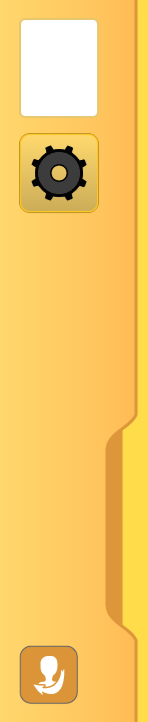
\includegraphics[width=0.1\textwidth]{sprint_one/enforce_design_guide_in_settings/button_inconsistency}
    \caption{Example of inconsistent Buttons}
    \label{fig:button_inconsistency}
\end{figure}

This motivated \emph{SW606F15} to create a graphical design document which enforces a standard for the GUI \todo{Maybe insert the design document in the appendix and refer to it}. Further more this design flaw was found in the GUI of the launcher which made us commit to the job of solving this problem



\begin{itemize}
	\item Actionbar in settings panel
	\item Switch user in settings panel
	\item Update logout button in home activity
\end{itemize}